

\subsection{Bugs Reproduced}
\label{eval-bugs}



Table \ref{tab-bugs} lists all the \numEval bugs\footnote{Given the limited
time and number of students.}   we have reproduced (4
Cassandra bugs).
We chose these \numEval bugs
(among the \numStudy bugs we studied) because the reports contain 
more detailed
descriptions about the bugs, the affected protocols, the affected code
version numbers, configuration setups, and the patches.  Table
\ref{tab-bugs} also shows the number of nodes needed for the bug symptoms
to surface and the quantifiable metrics of the symptoms.
%
Our first target system was Cassandra, hence the more bugs reproduced
compared to Riak and Voldemort; the latter two were added for  stronger
proof of concept.
%
Figure \ref{fig-bugs} shows the accuracy of \sck in reproducing the 6 bugs
using the metrics shown in Table \ref{tab-bugs}.
%
The first bug, \caone, has been described in \sec\ref{mot-bug} and
\sec\ref{eval-accu}.
%
We now briefly discuss the other five bugs 
(shown in Figure \ref{fig-bugs}) and then
%
make several important remarks.


Figure \ref{fig-bugs}a: In \catwo \cite{CA-Two}, 
when a node D is decommissioned from a
large cluster, all other nodes must own D's key-partitions.
This scale-dependent ``pending keyrange calculation'' is CPU intensive,
causing cluster-wide flapping, significantly observable in 256+ nodes.
The developers fixed it by caching outputs of slow methods.

Figure \ref{fig-bugs}b: \catri \cite{CA-Tri} 
is similar to the previous bug (\catwo),
but the fix was not efficient enough because in this new bug, the concept
of ``virtual nodes'' (multiple key-partitions per node) was added to
Cassandra.  The calculation is now scale-dependent to $N$$\times$$P$ and
becomes very CPU intensive.  This causes massive flapping during scaling out; 
the bug surfaced in 64+ nodes (when 32+ new nodes are added
to existing 32+ nodes). The bug was fixed with a complete 
redesign of the pending keyrange calculation.
%



\begin{table}
\begin{center}
\small
\centering
%---------------------------------
\begin{tabular}{l|r|l|l} 
{\bf Bug\#} & 
{\bf Surface} & 
{\bf Protocol} & {\bf Metric} \\
\hline
\caone \cite{CA-One} &$N$$\geq$256 & Bootstrap & \flaps \\
\catwo \cite{CA-Two}   & $\geq$256 & Decommission & \flaps \\
\catri \cite{CA-Tri}   & $\geq$64 & Add new nodes & \flaps \\
\cafour \cite{CA-Four}  & $\geq$256 & Add new nodes & \flaps \\
\riakone \cite{RIAK-One} & $\geq$128 & Boot+rebalance & $T_{Complete}$ \\
\voldone \cite{VOLD-One} & $\geq$128 & Rebalance & $T_{Complete} $ \\
\end{tabular}
%---------------------------------
\end{center}
\vminten
\mycaption{tab-bugs}{Reproduced bugs (\sec\ref{eval-bugs})}{``Surface'' 
implies the number of nodes
needed for the bug symptom to surface.
``c'' stands for Cassandra, ``r'' for Riak, and ``v'' for
Voldemort. 
}
\vminfive
\end{table}





Figure \ref{fig-bugs}c: Interestingly, \cafour \cite{CA-Four} is 
a bug in the {\em same}
protocol as in the previous bug.  We wondered why the previous fix does
not work here.  We found that pending range calculation is now
multi-threaded; different range calculations can happen concurrently.
This new design however introduces a new coarse-grained lock that creates
a new problem;  it can block gossip processing for a long
time, thus introduce flapping (in 256+ nodes).  The fix changed the
lock management.
%
The figure also shows that, for this workload, offline time profiling
is not fully accurate as the bug is order sensitive at large scale.
We are now testing it with order determinism. 


\if 0
Figure \ref{fig-bugs}d: In \voldone \cite{VOLD-One}, 
Voldemort's rebalancing was not
optimized for large clusters; it led to more stealer-donor partition
transitions as the cluster size grows (128+ nodes).  To fix this, the
developers completely changed the stealer-donor partition 
transition algorithm.
\fi


\if 0
Figure \ref{fig-bugs}e: In \riakone \cite{RIAK-One}, Riak bootstrapping
employed a complex 3-stage rebalancing algorithm (claim-target,
claim-hole, full-rebalance) that each node runs to eventually converge and
achieve a  perfect balance of the ring.  Each node runs this
CPU-intensive algorithm on {\em every} bootstrap gossip received.  The
larger the cluster, the longer time perfect balance is achieved (observed in
128+ nodes).
% This decentralized
% rebalancing was fixed with a centralized rebalancing.  
For Riak, we profile the rebalancing time along with pre-memoization (with
order determinism; \sec\ref{sc-pil-3}-\ref{sc-pil-4}).  Figure
\ref{fig-bugs}f (similar to Figure \ref{fig-accu}d) compares the execution
time of the rebalance function invocations in \sck and real deployments.
The figure shows that \sck's PIL exhibits a high accuracy.
\fi




\def \fgw {1.77in}


\begin{figure}[t]

\vminten

\centerline{
\hmina
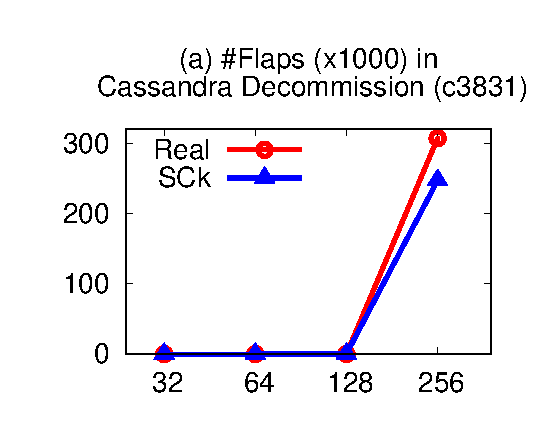
\includegraphics[width=\fgw]{F/old-bugs/eps/cass2.eps}
\hminb
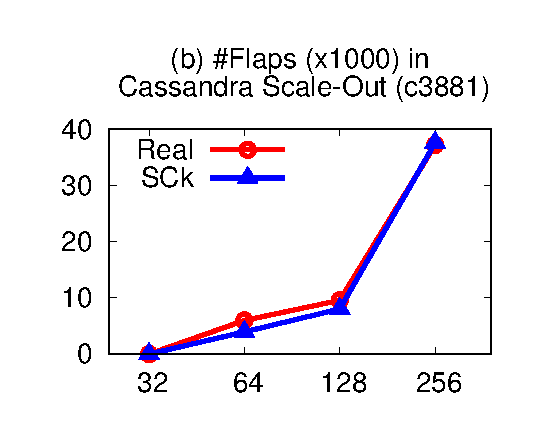
\includegraphics[width=\fgw]{F/old-bugs/eps/cass3.eps}
\hmina
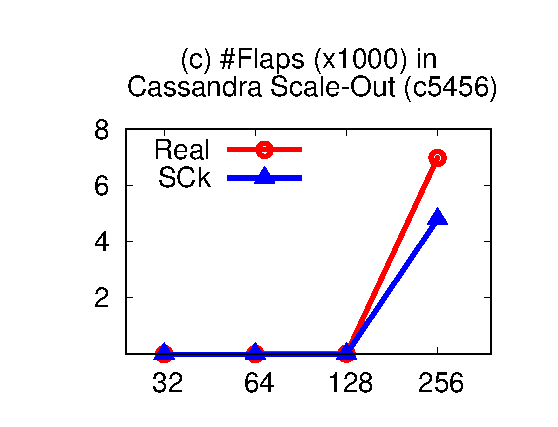
\includegraphics[width=\fgw]{F/old-bugs/eps/cass4.eps}
}
%\centerline{
%\hmina
%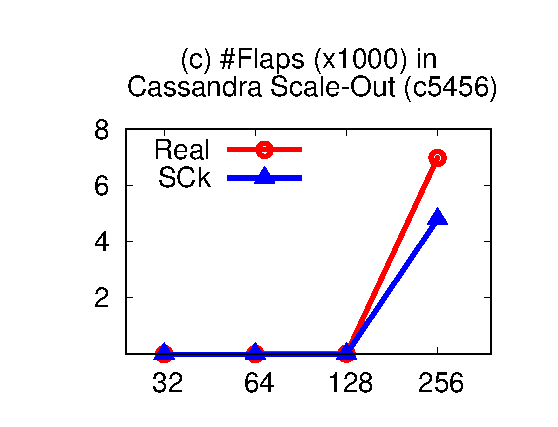
\includegraphics[width=\fgw]{F/old-bugs/eps/cass4.eps}
%\hminb
%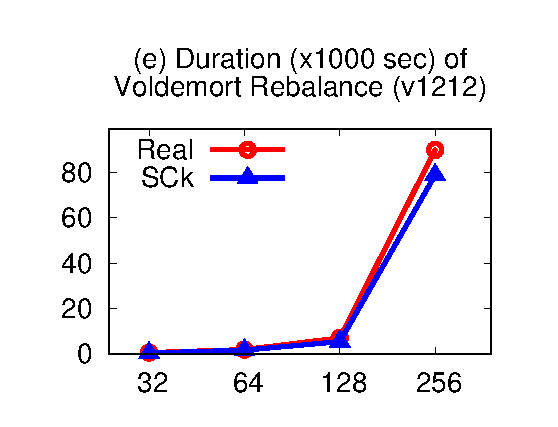
\includegraphics[width=\fgw]{F/old-bugs/eps/vold1.eps}
%}

%\centerline{
%\hmina
%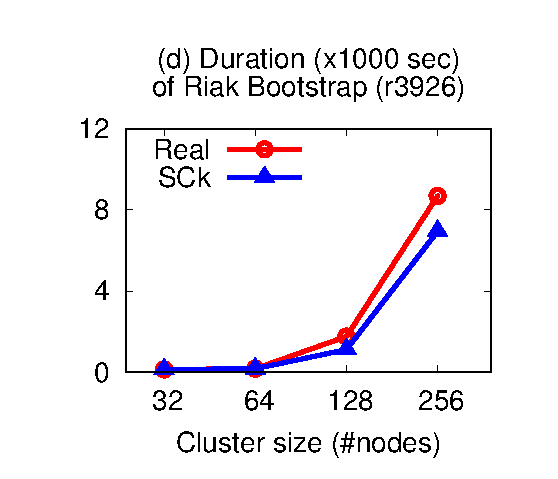
\includegraphics[width=\fgw]{F/old-bugs/eps/riak1.eps}
%\hminb
%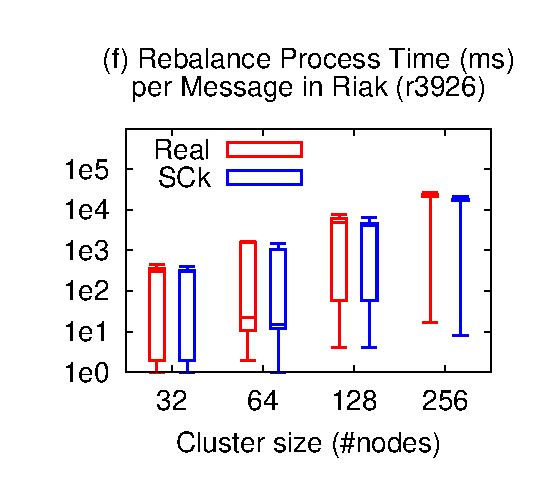
\includegraphics[width=\fgw]{F/riak/eps/proc.eps}
%}

\vminfive

\mycaption{fig-bugs}{Accuracy in reproducing other 
bugs (\sec\ref{eval-bugs})}{The
figures represent the bugs described in Table \ref{tab-bugs}.  
The title represents the y-axis. 
We cap the y-axis to show the scale at which the bug symptoms start
to appear. }
\vminfive
\end{figure}



\if 0

TODO: CASS2: waiting for NOme to go up.
Meanwhile doing CASS3. 
%
RIAK: Buggy done, but need to plug in data from new version
(Cesar is adding fixed/patched line from the newest version).
%
VOLD: (Wait until all features are in).  Still running.
\fi




We make several remarks from this experience.
%
First, if \sck had existed in the first place, it might have {\em
  prevented} the Cassandra bugs; they all involve the same protocols
(gossip, rebalance, and failure detector) and create the same symptom
(high \flaps).  These bugs highlight that code evolution can introduce new
bugs in the same protocols.  In this context, \sck is highly useful.
%
Second, reproducing scalability bugs is relatively {\em easy} as we
achieve a high colocation factor.  Unlike non-deterministic bugs which
require complex timing reordering to reproduce 
\cite{Guo+11-Demeter, Leesatapornwongsa+14-Samc},
% \cite{Leesatapornwongsa+16-TaxDC},
symptoms of scalability bugs are ``deterministically scale-dependent.''
%
%
Third, different systems of the same type (\eg, key-value
store) implement similar protocols.  The {\em generality} of \sck methods
in scale-checking the protocols above can be useful to many other
distributed key-value stores.




% https://mail.google.com/mail/u/0/#inbox/1544ecd936258917


